\documentclass{standalone}
\usepackage{mtpro2}
\usepackage{tikz}
\usetikzlibrary{calc,patterns,decorations.pathmorphing,decorations.markings}

\begin{document}
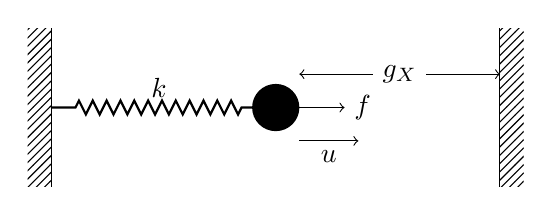
\begin{tikzpicture}[scale=1.5]
\tikzstyle{spring}=[thick,decorate,decoration={zigzag,pre length=0.3cm,post length=0.3cm,segment length=5}]
\tikzstyle{ground}=[fill,pattern=north east lines,draw=none,minimum width=0.75cm,minimum height=0.3cm]
% ========= bucks
\node (wall) [ground, minimum width=.3cm, minimum height=2cm] {};
\draw (wall.north east) -- (wall.south east);

\node (mass1) at (2,0) {};
\fill (mass1) circle (.2);

\node (wall2) at (4,0) [ground, minimum width=.3cm, minimum height=2cm] {};
\draw (wall2.south west) -- (wall2.north west);
% ====== connections
\draw [spring] (wall) -- node [above] {$k$} (mass1);
%% ===== comments
\draw [<->] (mass1.north) ++ (.2,.2) -- node [fill=white] {$g_X$} +(1.7,0);
\draw [->] (mass1.south) ++ (.2,-.2) -- node [below] {$u$} +(1/2,0) ;
\draw [->] (mass1.east) -- +(1/2,0) node [right] {$f$};
%\draw [<-] (wall2.west)  -- node [above] {$\lambda$} +(1,0) ;
\end{tikzpicture}
\end{document}
